\documentclass{article}

% if you need to pass options to natbib, use, e.g.:
%     \PassOptionsToPackage{numbers, compress}{natbib}
% before loading neurips_2019

% ready for submission
% \usepackage{neurips_2019}

% to compile a preprint version, e.g., for submission to arXiv, add add the
% [preprint] option:
%     \usepackage[preprint]{neurips_2019}

% to compile a camera-ready version, add the [final] option, e.g.:
\usepackage[preprint]{neurips_2019}

% to avoid loading the natbib package, add option nonatbib:
%     \usepackage[nonatbib]{neurips_2019}

\usepackage[utf8]{inputenc} % allow utf-8 input
\usepackage[T1]{fontenc}    % use 8-bit T1 fonts
\usepackage{hyperref}       % hyperlinks
\usepackage{url}            % simple URL typesetting
\usepackage{booktabs}       % professional-quality tables
\usepackage{amsfonts}       % blackboard math symbols
\usepackage{amsmath}
\usepackage{nicefrac}       % compact symbols for 1/2, etc.
\usepackage{microtype}      % microtypography
\usepackage{color}
\usepackage{graphicx}

\setcitestyle{numbers}
\setcitestyle{square}
\setcitestyle{comma}
\bibliographystyle{abbrvnat}
\setlength{\bibsep}{4pt plus 2pt minus 2pt}

\newcommand{\bx}{\mathbf{x}}
\newcommand{\bv}{\mathbf{v}}
\newcommand{\bm}{\mathbf{m}}
\newcommand{\bb}{\mathbf{b}}

\newcommand{\todo}[1]{\textcolor{red}{TODO: #1}}



\title{Scalable Extreme Deconvolution}

% The \author macro works with any number of authors. There are two commands
% used to separate the names and addresses of multiple authors: \And and \AND.
%
% Using \And between authors leaves it to LaTeX to determine where to break the
% lines. Using \AND forces a line break at that point. So, if LaTeX puts 3 of 4
% authors names on the first line, and the last on the second line, try using
% \AND instead of \And before the third author name.

\author{
  James A. Ritchie\\
  School of Informatics\\
  University of Edinburgh\\
   \texttt{james.ritchie@ed.ac.uk} \\
  \And
  Iain Murray\\
  School of Informatics\\
  University of Edinburgh\\
   \texttt{i.murray@ed.ac.uk} \\
}

\begin{document}

\maketitle

\begin{abstract}

The Extreme Deconvolution method fits a probability density to a dataset where every observation has Gaussian noise added with a known sample-specific covariance, originally intended for use with astronomy datasets.
The existing method of fitting the model cannot scale to new larger astronomy datasets.
We propose two extensions to the extreme deconvolution method based on an online variation of the EM algorithm, and direct optimisation of the log-likelihood via minibatch gradient descent, both of which can make use of GPU computation.
We demonstrate that these methods provide faster fitting of the model, whilst being able to scale to much larger datasets.

\end{abstract}

\section{Introduction}

Extreme deconvolution is a method that fits Gaussian Mixture Models (GMM)s to noisy data where we know the covariance of the Gaussian noise added to each sample~\cite{bovyExtremeDeconvolutionInferring2011}.
The method was originally developed to perform probabilistic density estimation on the dataset of stellar velocities produced by the Hipparcos satellite~\cite{perrymanHipparcosCatalogue1997}.
The Hipparcos catalogue consists of astrometric solutions (positions and velocities on the sky) and photometry (light intensity) for 118,218 stars, with associated noise covariances provided for each entry.

The successor to the Hipparcos mission, Gaia, aims to produce an even larger catalogue, with entries for an estimated 1 billion astronomical objects~\cite{collaborationGaiaMission2016}.
Previous work using an extreme deconvolution model on the Gaia catalogue had to work with a subset of the data, as the existing method of fitting the models cannot work with very large datasets \cite{andersonImprovingGaiaParallax2018}.
It must make a full pass over the dataset before it can update parameters, and the reference implementation requires all the data to fit in memory.

In this work, we propose two new methods for fitting the extreme deconvolution model that can scale to the full dataset size, based on an online variation of the Expectation-Maximisation (EM) algorithm, and minibatch gradient descent on the log-likelihood.
We develop implementations that can leverage GPU-based computation, and show that they provide comparable density estimates to the existing method, whilst being much faster to train.

\section{Background}

The aim of extreme deconvolution is to perform density estimation on a noisy $d$-dimensional dataset $\{\bx_i\}_{i=0}^N$, where $\bx_i$ was generated by adding zero-mean Gaussian noise $\epsilon_i$ with known per-datapoint covariance $S_i$ to a projection $R_i$ of a true value $\bv_i$,
\begin{equation}
  \bx_i = R_i\bv_i + \epsilon_i,\quad  \epsilon_i \sim \mathcal{N}(\mathbf{0}, S_i).
\end{equation}
We assume that $\bv_i$ can be modelled by a mixture of Gaussians with $K$ components,
\begin{equation}
p(\bv_i \mid \theta) = \sum_j^K \alpha_j \mathcal{N}(\bv \mid \bm_j, V_j), \quad \theta = \{\alpha_j, \bm_j, V_j\}_{j=1} ^ K
\end{equation}
As both the noise model is Gaussian and the density estimation model is a mixture of Gaussians, the likelihood of $\bx_i$ is also a Gaussian mixture,
and the total log-likehood of the dataset is
\begin{equation}
\mathcal{L}(\theta) = \sum_i^N \log \sum_j^K \alpha_j\mathcal{N}(\bx_i \mid R_i\bm_j, T_{ij}), \quad T_{ij} = R_iV_jR_i^T + S_i.
\end{equation}

Missing data can be handled either by making $R_i$ rank-deficient, or by setting elements of the covariance matrix $S_i$ to very large values.

\section{Methods}

\subsection{Minibatch Expectation-Maximisation}

The original method of fitting the extreme deconvolution model used a modification of the Expectation-Maximisation (EM) algorithm for mixture models~\cite{dempsterMaximumLikelihoodIncomplete1977}.
Here we describe a minibatch version of this algorithm based on~\citet{cappeOnlineExpectationMaximization2009}'s online EM algorithm for latent data models.
At each iteration $t$, we compute the sufficient statistics of the latent data $\bv_i$ for each component $j$ in the minibatch of size $M$, using our current estimate of the parameters,
\begin{equation}
r_{ij} = \frac{\alpha_j \mathcal{M}(\bx_i \mid R_i\bm_j, T_{ij})}{\sum_k \alpha_k \mathcal{N}(\bx_i \mid R_i\bm_k, T_{ik})}, \ 
\bb_{ij} = m_j + V_j R_i^T T_{ij}^{-1}(\bx_i - R_i \bm_j), \ 
B_{ij} = V_j - V_j R_i^T T_{ij}^{-1}R_iV_j.
\end{equation}
The $r_{ij}$ term is just the posterior probability of datapoint $\bx_i$ coming from component $j$.
The $\bb_{ij}$ and $B_{ij}$ terms result from the fact that $\bx_i$ and $\bv_i$ are jointly Gaussian, so the distribution of $\bv_i$ conditioned on $\bx_i$ is also Gaussian with mean $\bb_{ij}$ and covariance $B_{ij}$.
The expected sufficient statistics are then summed together over the minibatch,
\begin{equation}
\phi_j^1 = \sum_i r_{ij}, \quad
\phi_j^2 = \sum_i r_{ij} \bb_{ij}, \quad
\phi_j^3 = \sum_i r_{ij} [\bb_{ij}\bb_{ij}^T + B_{ij}].
\end{equation}
Stochastic estimates $\hat{\phi}_{tj} $ of the sums of sufficient statistics over the whole dataset are then updated with a sufficiently small step size $\lambda$,
\begin{equation}
\hat{\phi}_{tj} = (1 - \lambda)\hat{\phi}_{(t-1)j} + \lambda \phi_{tj}.
\end{equation}
Finally, we normalise the updated sums of expected sufficient statistics to get updated estimates of the parameters.
\begin{equation}
\alpha_j = \frac{\hat{\phi}_j^1}{M}, \quad
\bm_j = \frac{\hat{\phi}_j^2}{\hat{\phi}_j^1}, \quad
V_j = \frac{\hat{\phi}_j^3}{\hat{\phi}_j^1} - \bm_j \bm_j^T.
\end{equation}
This procedure is repeated with new randomly ordered minibatches until convergence.
If we set $\lambda=1$, replace each minibatch with the entire dataset and factorise the update for $V_j$ then we recover the original fitting method.
The update for $V_j$ could result in catastrophic cancellation if the variances of the components are small relative to the means, especially if single precision floats are used, as is standard with GPU computation.
In Appendix~\ref{apx:variance-rewrite} we show how this update can be rewritten in a symbolically equivalent but more numerically stable form.


\subsection{Stochastic Gradient Descent}

An alternative to EM-based methods is to optimise the log-likelihood directly.
The log-likelihood has some constraints on its parameters, namely that the weight $a_j$ sum to $1$ and that the covariances $V_j$ are positive definite.
Directly fitting it with standard gradient-based optimisers requires a transformation of the parameters to remove the constraints.
The mixture weights $\alpha_j$ can be parameterised by taking the softmax of an unconstrained vector $\mathbf{z}$, and the covariances $V_j$ as a lower triangular matrix $L_j$ via the Cholesky decomposition, where the diagonal elements $qq$ of $L_j$ are constrained positive by taking the exponential of the unconstrained element $\tilde{L}_q$,
\begin{equation}
\alpha_j = \frac{e^{z_j}}{\sum_{k=1}^K e^{z_k}}, \quad
V_j = L_jL_j^T, \quad
(L_j)_{qq} = \exp({\tilde{L}_q}).
\end{equation}
Note that for a standard GMM we could bypass forming the covariance altogether and evaluate the log PDF of the Normal distribution directly with the Cholesky factor.
For the extreme deconvolution model, this cannot be done, as we need to form the covariance $Tij$ for every datapoint.
Having removed the constraints, we can then take the gradient of the log-likelihood with respect to the parameters and optimise it using a standard minibatch-based optimiser.

\section{Experiments}

We implemented both of our methods in PyTorch, and compared against the reference implementation from \citet{bovyExtremeDeconvolutionInferring2011}.
To evaluate each method, we used a random sample of rows from the Gaia DR2 source table~\cite{brownGaiaDataRelease2018}.
We selected the 5 primary astrometric features, along with the BP-RP colour and mean magnitude in the G-band.
In total there were 2 million rows.
Where data were missing, we set the field to zero and the noise variance to a large value.
We set the projection $R_i$ to the identity matrix for every sample.
This is only a small fraction of the full dataset size, but this allows us to fit the training data into memory, a requirement for use with the original implementation of extreme deconvolution.
We used a range of mixture component sizes $K$.
In practice we would want to select a value of $K$ by cross-validation.

Initialisation of all models was performed by first running a minibatch version of the K-means clustering algorithm on the dataset to get estimates of the weights and means \cite{sculleyWebscaleKmeansClustering2010}.
Initial covariances were set to the identity matrix.
Training was done for 20 epochs.
The existing EM method ran on CPU, whilst the minibatch EM and SGD methods ran on GPU.
We used a validation set comprising $10\%$ of the rows when developing our experiments.
Final model performance was evaluated on a different held-out test set also comprising 10\% of the rows at the last stage, with no parameter selection or development done based on this value.
Table~\ref{results-table} reports the validation and test log-likelihoods for each method along with average training time.
Figure~\ref{fig:training} plots the training log-likelihood against time-rescaled epoch for $K=256$ and training time as function of mixture components $K$.
Figure~\ref{fig:projection} shows a 2-D projection from an example model with $K=256$ fitted with the minibatch-EM method.

\begin{table}{}
  \caption{Average validation and test log-likelihoods with average training time for the Gaia data subset for different numbers of mixture components $K$.  Average over 5 runs with standard deviation.}
  \label{results-table}
  \centering
  \begin{tabular}{lcccc}
    \toprule
    Method     & K &  Validation     & Test & Time (minutes) \\
    \midrule
    Existing EM                                     & 64  & $-26.12 \pm 0.03$ & - & $60.0 \pm 7.9$\\
    (\citet{bovyExtremeDeconvolutionInferring2011}) & 128 & $-25.95 \pm 0.04$  & - & $101.1 \pm 2.19$    \\
                                                    & 256 & $-25.76 \pm 0.02$ & - & $195.3 \pm 4.08$ \\
    \midrule
    Minibatch EM  & 64  & $-26.04 \pm 0.01$   & - & $26.8 \pm 1.71$ \\
                  & 128 & $-25.92 \pm 0.01$   & - & $44.5 \pm 1.0$      \\
                  & 256 & $-25.83 \pm 0.003$  & - & $51.6 \pm 3.0$ \\
    \midrule
    SGD & 64    & $-26.10 \pm 0.02$  & - &$23.5 \pm 2.34$ \\
        & 128   & $-25.94 \pm 0.01$  & - & $34.0 \pm 0.83$ \\
        & 256   & $-25.84 \pm 0.01$  & - & $36.6 \pm 1.3$ \\
    \bottomrule
  \end{tabular}
\end{table}

\begin{figure}
  \centering
  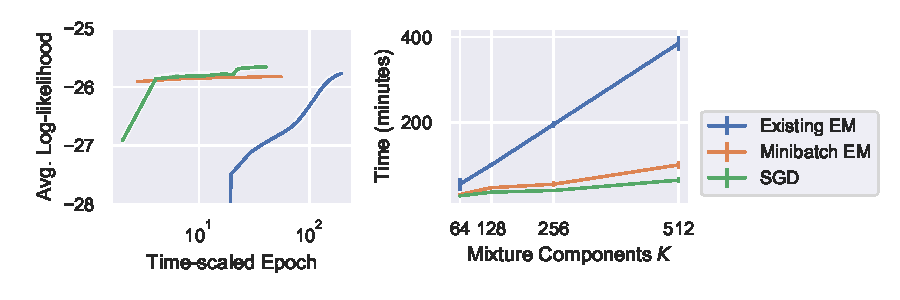
\includegraphics{learning.pdf}
  \caption{\textbf{Left}: Average training log-likelihood as a function of training epoch for models with $K=256$. Epochs rescaled by average training time. Error bars not visible. \textbf{Right}: Training time as a function of mixture components $K$. Error bars indicate $\pm$ 2 standard deviations.}
  \label{fig:training}
\end{figure}

\begin{figure}
  \centering
  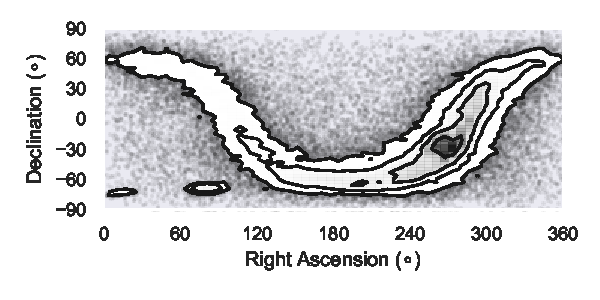
\includegraphics{density.pdf}
  \caption{Density plot showing a 2-D projection of 100000 samples drawn from a model with $K=256$ and fitted with the minibatch EM method.
  The plot shows the estimated density of star positions on the sky, and has correctly recovered the structure of the Milky Way and the Magellanic Clouds.}
  \label{fig:projection}
\end{figure}

\section{Discussion}

Our results have shown that both of our proposed methods perform comparably to the existing method of fitting extreme deconvolution models, whilst being able to work with datasets that cannot fit in memory.
The results also show that using GPU-based computation speeds up training considerably as mixture component size $K$ increases.

Further improvements to our approaches are possible.
The original paper presents a method of getting out of local maxima by splitting and merging clusters, with the split-merge criteria evaluated on the whole dataset.
It should be possible to replace the criteria with stochastic estimates, which would permit them to be used with both the SGD and minibatch EM methods.
Our approaches also add more free parameters to be selected, including learning rate and batch size.
This adds scope for hyperparameter optimisation to improve the log-likelihood, potentially making use of Bayesian optimisation.

The question remains of which method should be used for any particular problem?
The existing EM method had comparable log-likelihoods for smaller sizes of $K$, and did marginally better for the largest size, but at the cost of a much longer training time.
The SGD method is faster than the minibatch EM method, especially as $K$ increases, at a cost of having a slightly worse log-likelihood.
The answer will therefore depend on exactly what dataset we wish to perform density estimation on, and how accurate an estimation we require.
In practice we would suggest using the minibatch EM method for relatively smaller datasets, and the SGD method on larger datasets.

\bibliography{references}

\appendix

\section{Stable Variance Update}
\label{apx:variance-rewrite}

\section{Experiment Details}

\end{document}
